\subsection{Red Subte}

Para el último experimento, capturamos los paquetes de la LAN Wi-Fi Subte-BA de la estación Plaza Italia de la Línea D del Subte de Buenos Aires.La medición fue realizada un día Domingo a las 16.30hs y durante solamente 1 minuto. La cantidad de paquetes capturados es de 1.000.

\begin{figure}[H]
       \centering
       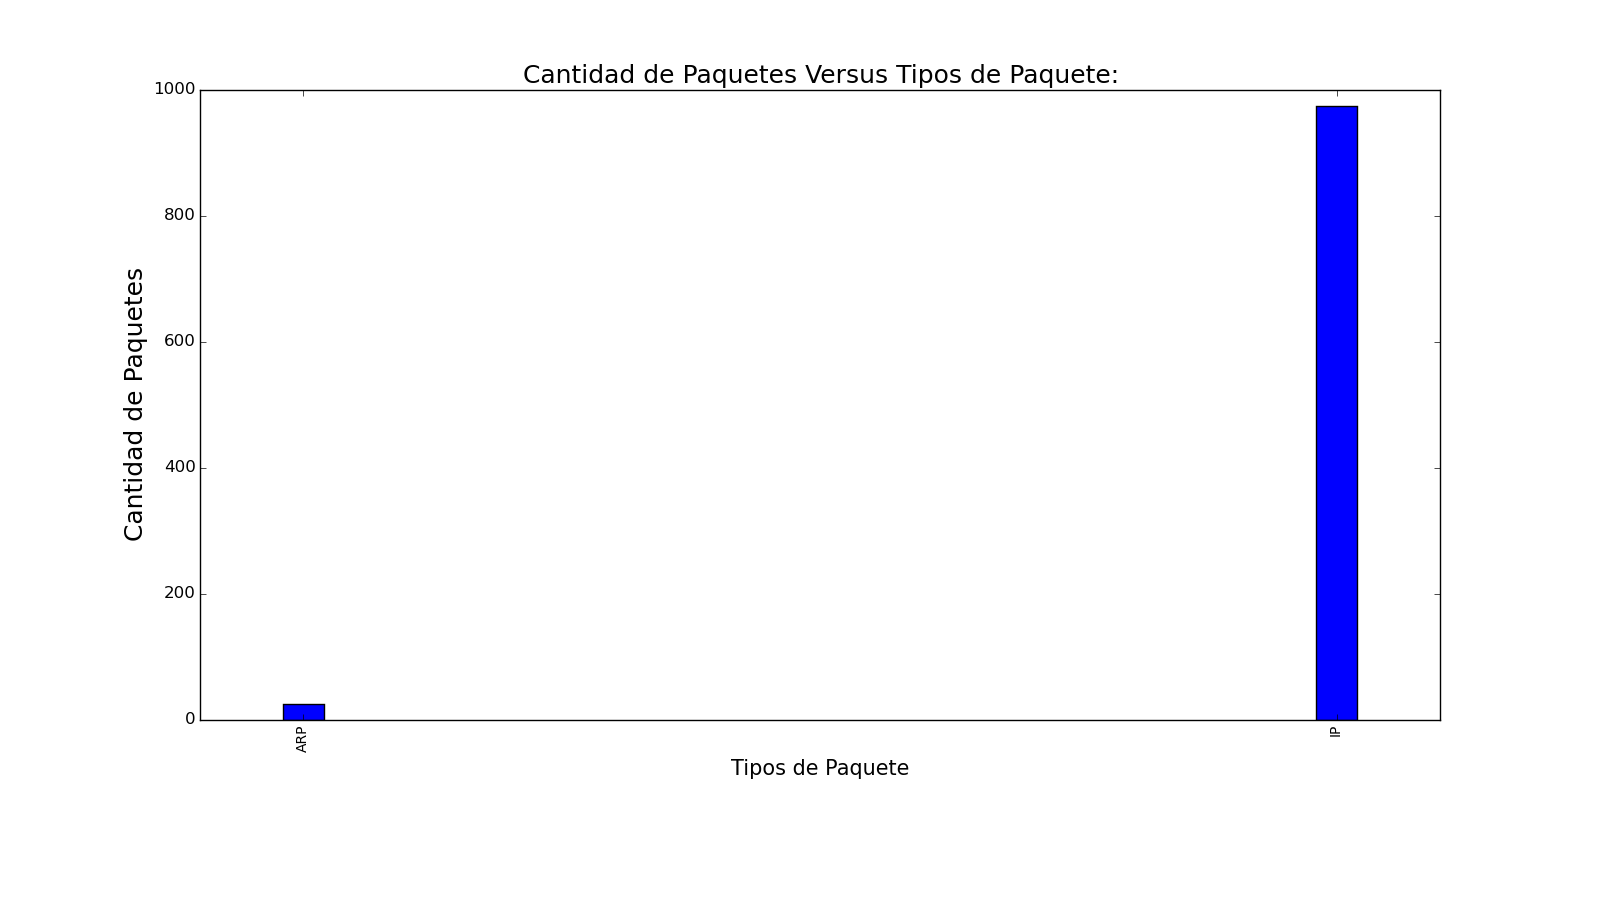
\includegraphics[width=1\textwidth]{../resultados/subte/histogram_types.png}
       \caption{Protocolos de los paquetes capturados}
       \label{red-hogarena-types}
\end{figure}

\begin{figure}[H]
       \centering
       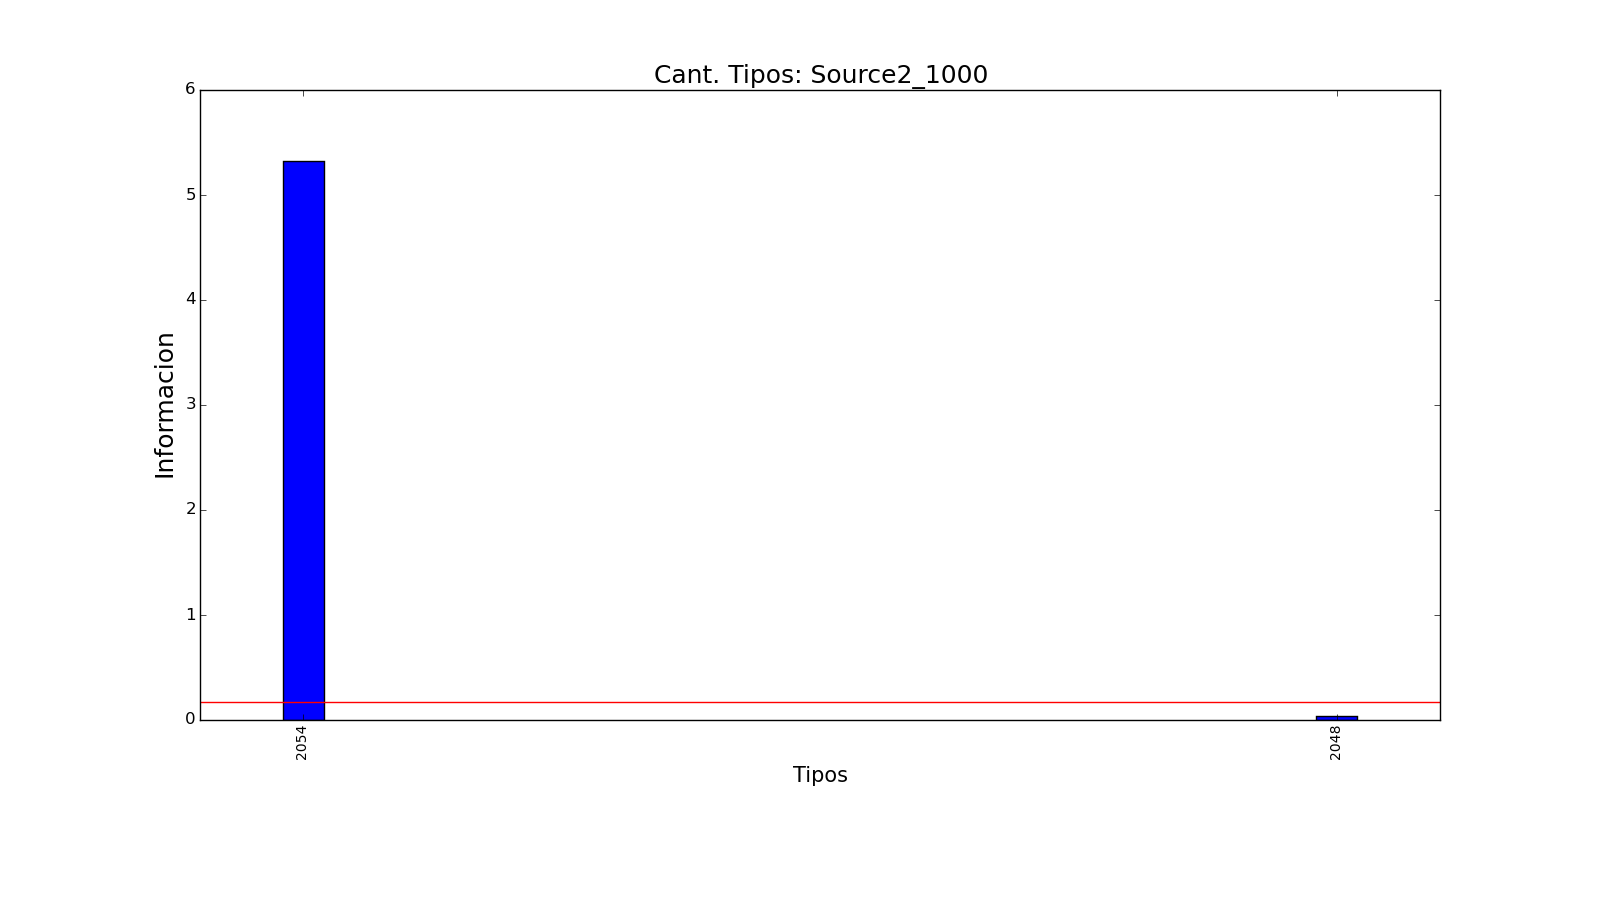
\includegraphics[width=1\textwidth]{../resultados/subte/histogram_types_information.png}
       \caption{Información de los protocolos de los paquetes capturados}
       \label{red-hogarena-types-info}
\end{figure}


\begin{figure}[H]
       \centering
       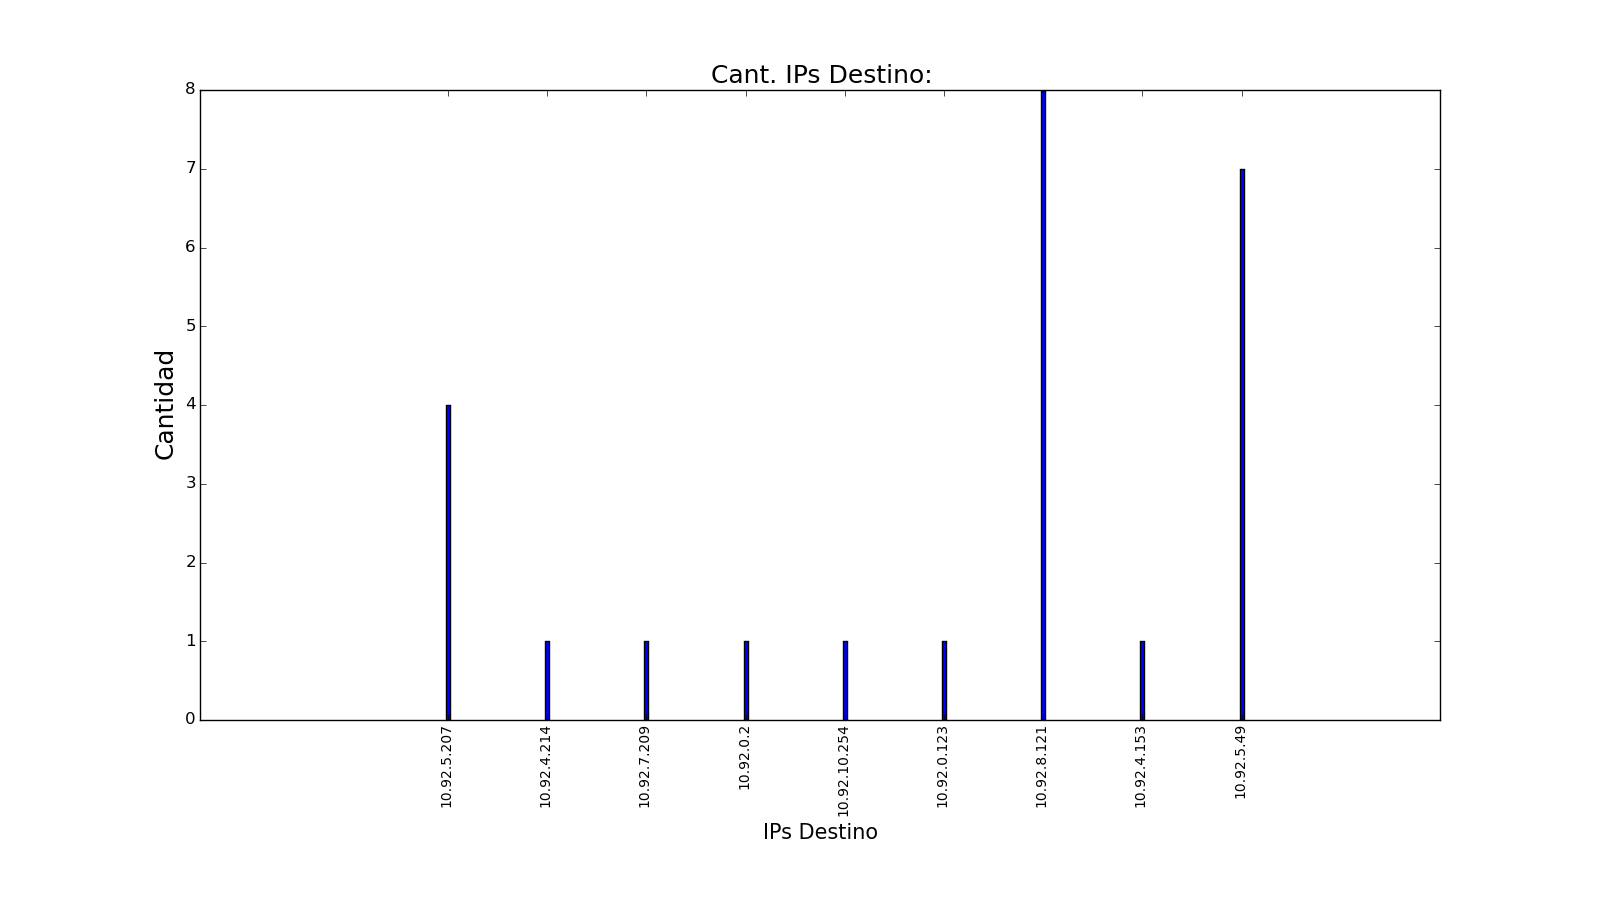
\includegraphics[width=1\textwidth]{../resultados/subte/histogram_dst.png}
       \caption{IPs destino de los paquetes ARP}
       \label{red-hogarena-arp-destination}
\end{figure}

\begin{figure}[H]
       \centering
       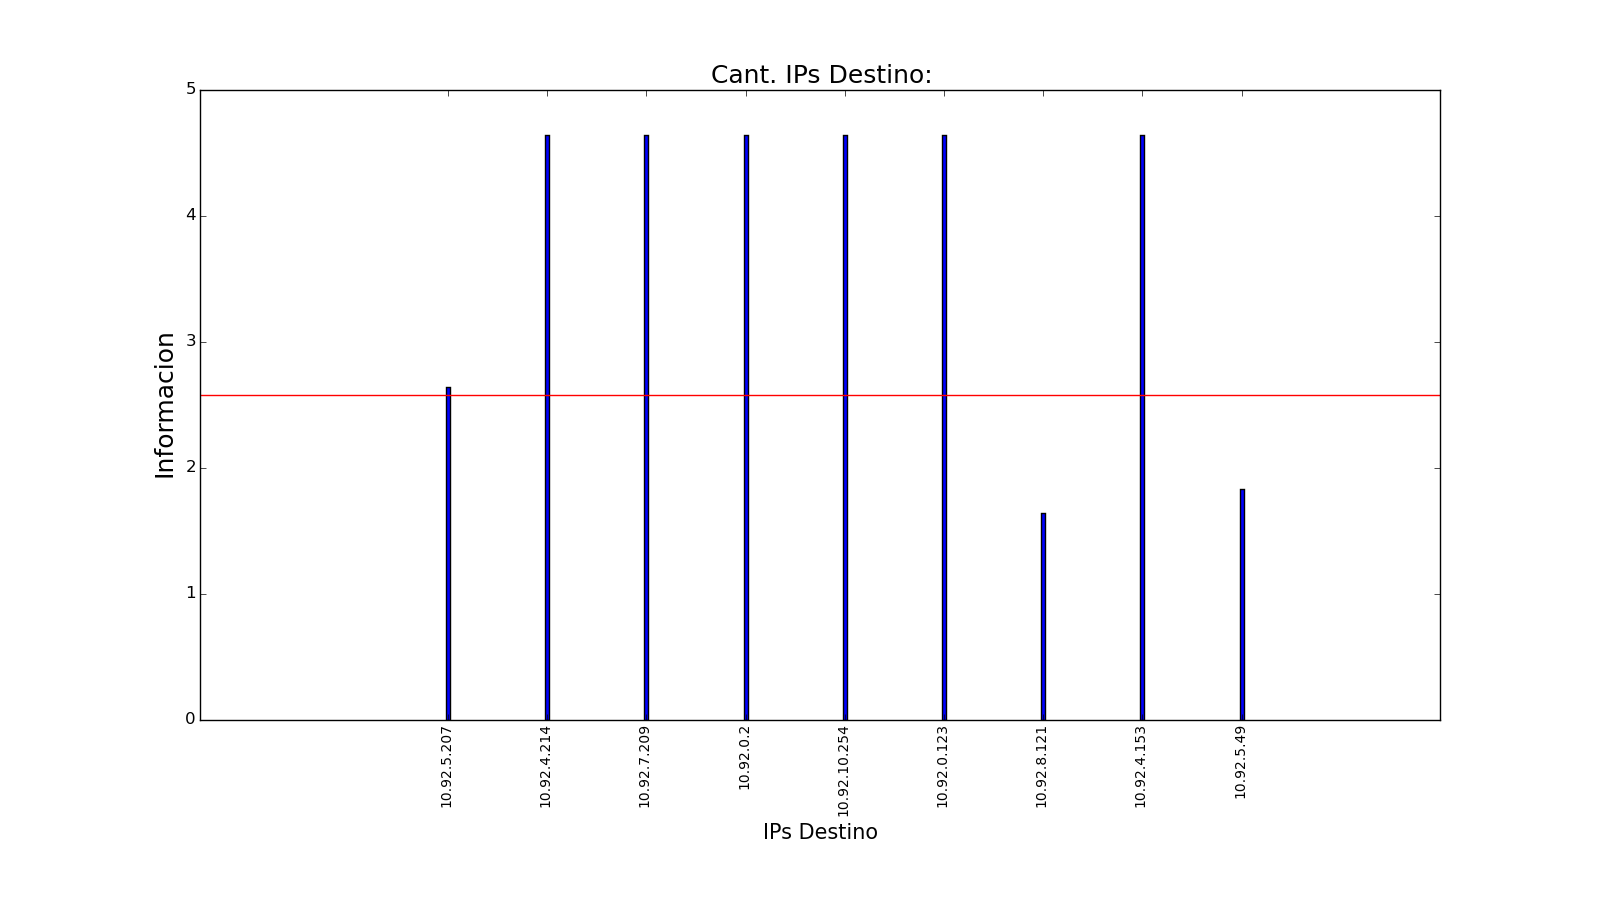
\includegraphics[width=1\textwidth]{../resultados/subte/histogram_dst_information.png}
       \caption{Información de IPs destino de los paquetes ARP}
       \label{red-hogarena-arp-destination-info}
\end{figure}

\begin{figure}[H]
       \centering
       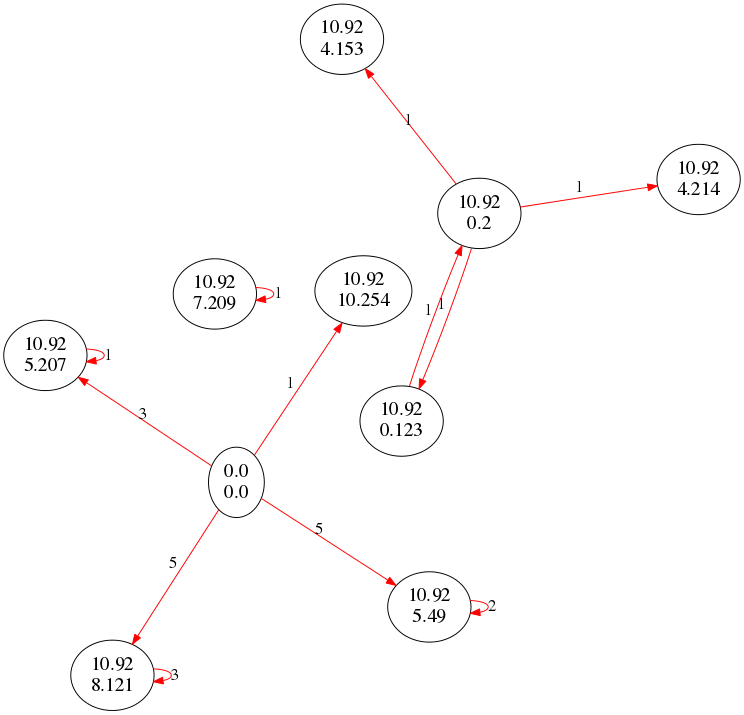
\includegraphics[width=1\textwidth]{../resultados/subte/network.png}
       \caption{Tráfico de paquetes ARP}
       \label{red-hogarena-arp-traffic}
\end{figure}